\section{\glsfmtlong{VSL}}
\label{sec:VSL}

The \glsfirst{VSL} is an Ethereum Layer 2 blockchain built with OP Stack uisng Celestia as the data availability layer.
It is responsible for handling value derived from \glsfmtlong{OI} activities and applications, establishing a healthy ownership economy for the Network.

The \glsfmtlong{R3N} allocates a portion of \$RSS3 total supply to incentivize network participants on the \gls{VSL}, this is known as the Network Rewards.
The Network Rewards is allocated into two reward pools: the \glsfirst{OP} and the \glsfirst{SP} for Normal Nodes, or the \glsfirst{PGP} for Public Good Nodes. See \Cref{fig:network-rewards}.

{
\begin{figure}[tb!]
    \centering
    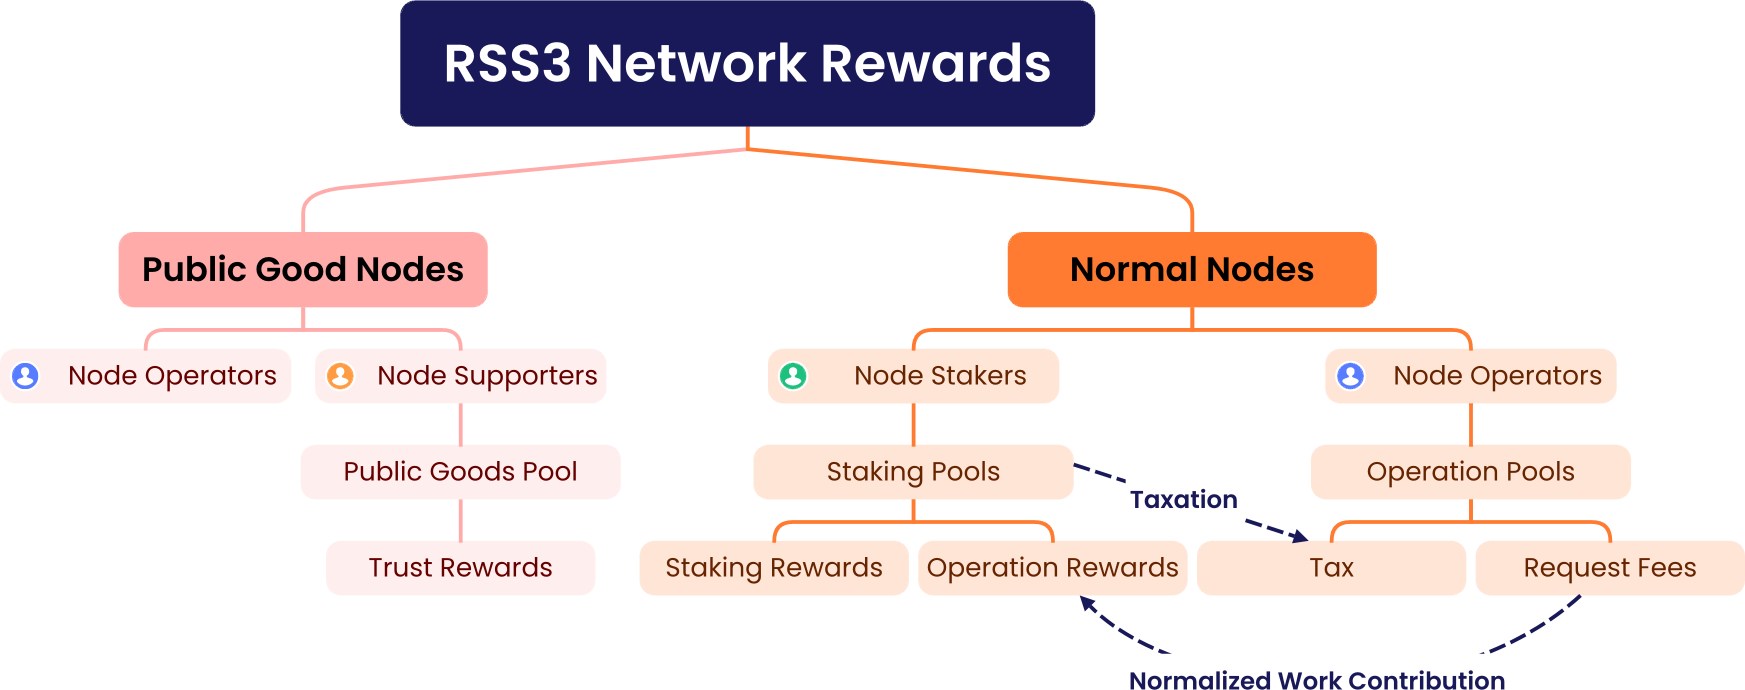
\includegraphics[width=0.8\columnwidth]{figures/network-rewards.png}
    \caption{RSS3 Network Rewards distribution.}
    \label{fig:network-rewards}
\end{figure}
}

The incentive mechanism of the \gls{VSL} is designed to encourage the following behaviors:

\subsubsection{Node Operation}
Nodes are incentivized to operate and maintain the Network by receiving \$RSS3 as rewards.
\begin{enumerate}
    \item Anyone can become a \glsfmtlong{NO} to launch an RSS3 Node and join the RSS3 Network without requiring prior permission.
    \item A \glsfmtlong{NO} has the ability to configure Node's coverage, which directly influences the Node's capability to respond to various types of requests. A broader coverage means more computational resources are required, and a higher chance of receiving requests.
    \item A Node can be operated in either a Normal mode or a Public Good mode. A Normal Node is eligible for network rewards, but requires a deposit of \$RSS3. A Public Good Node is ineligible for network rewards, but requires no deposit.
    \item A Normal Node has a corresponding \glsentrysymbol{OP} and a \glsentrysymbol{SP}. All Public Good Nodes collectively share a single \glsentrysymbol{PGP}.
\end{enumerate}

\subsubsection{Node Staking}
Network participants are incentivized to stake \$RSS3 to secure the Network by receiving \$RSS3 as rewards.
\begin{enumerate}
    \item A Normal Node accepts staking into its Reward Pool, the amount of staked \$RSS3 signifies its quality. Higher quality Nodes handle more requests.
    \item A Public Good Node does not have a Reward Pool and does not participate in any form of incentivization. Staking into a \glsfmtlong{PGP} is accepted, and the stakers can assign their trust to any Public Good Node. Higher trust Nodes handle more requests.
\end{enumerate}

{
\renewcommand{\arraystretch}{1.5}
\begin{table*}[h]
    \resizebox{\textwidth}{!}{
        \begin{tabulary}{\textwidth}{|p{6cm}|p{5cm}|p{5cm}|}
            \hline
            & \textbf{Node in Normal Mode} & \textbf{Node in Public Good mode} \\ \hline
            Who can operate? & Anyone & Anyone \\ \hline
            Can operators specify the coverage? & Yes & Yes \\ \hline
            Is a deposit required? & Yes & No \\ \hline
            Is the deposit considered as staking, making it eligible for rewards from the Reward Pool & No & N/A \\ \hline
            Will the Node be slashed? & Yes, the deposit and its \gls{SP} will be slashed. A Node may be demoted to receive fewer requests. & No, but a Node may be demoted to receive fewer requests. \\ \hline
            Does the Node accept staking? & Yes. The staked tokens go to the Node’s Reward Pool. RSS3-X (X being the Node’s name) Chips are issued to the stakers after staking. & No, as such a Node does not have a Reward Pool. Instead, stakers stake to a Public Good Pool. RSS3-Public Good Chips are issued to the stakers after staking. \\ \hline
            Can operators set a tax? & Yes & No, a universal tax is set by DAO. \\ \hline
            Can operators participate in Governance? & Yes & Yes, limited to Public Good proposals. \\ \hline
            Does it have an Operator Pool? & Yes & No, operator rewards go to [X] \\ \hline
            Does it have a Reward Pool? & Yes & No, but a Public Good Pool with a universal incentive rate set by DAO. \\ \hline
        \end{tabulary}
    }
    \caption{Comparison of two Node operation modes.}
    \label{table:node_modes}
\end{table*}
}